\documentclass[a4paper,11pt]{exam}
\printanswers % pour imprimer les réponses (corrigé)
%\noprintanswers % Pour ne pas imprimer les réponses (énoncé)
\addpoints % Pour compter les points
% \noaddpoints % pour ne pas compter les points
%\qformat{\textbf{\thequestion ) } }
%\qformat{\textbf{\thequestion )} (\thepoints) \\} % Pour définir le style des questions (facultatif)
\usepackage{color} % définit une nouvelle couleur
\shadedsolutions % définit le style des réponses
% \framedsolutions % définit le style des réponses
\definecolor{SolutionColor}{rgb}{0.8,0.9,1} % bleu ciel
\renewcommand{\solutiontitle}{\noindent\textbf{Solution:}\par\noindent} % Définit le titre des solutions




\makeatletter

\def\maketitle{{\centering%
	\par{\huge\textbf{\@title}}%
	\par{\@date}%
	\par}}

\makeatother

\lhead{NOM Pr\'enom :}
\rhead{\textbf{Les r\'eponses doivent \^etre justifi\'ees}}
\cfoot{\thepage / \pageref{LastPage}}


%\usepackage{../../pas-math}
%\usepackage{../../moncours}


%\usepackage{pas-cours}
%-------------------------------------------------------------------------------
%          -Packages nécessaires pour écrire en Français et en UTF8-
%-------------------------------------------------------------------------------
\usepackage[utf8]{inputenc}
\usepackage[frenchb]{babel}
\usepackage[T1]{fontenc}
\usepackage{lmodern}
\usepackage{textcomp}



%-------------------------------------------------------------------------------

%-------------------------------------------------------------------------------
%                          -Outils de mise en forme-
%-------------------------------------------------------------------------------
\usepackage{hyperref}
\hypersetup{pdfstartview=XYZ}
%\usepackage{enumerate}
\usepackage{graphicx}
\usepackage{multicol}
\usepackage{tabularx}
\usepackage{multirow}


\usepackage{anysize} %%pour pouvoir mettre les marges qu'on veut
%\marginsize{2.5cm}{2.5cm}{2.5cm}{2.5cm}

\usepackage{indentfirst} %%pour que les premier paragraphes soient aussi indentés
\usepackage{verbatim}
\usepackage{enumitem}
\usepackage[usenames,dvipsnames,svgnames,table]{xcolor}

\usepackage{variations}

%-------------------------------------------------------------------------------


%-------------------------------------------------------------------------------
%                  -Nécessaires pour écrire des mathématiques-
%-------------------------------------------------------------------------------
\usepackage{amsfonts}
\usepackage{amssymb}
\usepackage{amsmath}
\usepackage{amsthm}
\usepackage{tikz}
\usepackage{xlop}
%-------------------------------------------------------------------------------



%-------------------------------------------------------------------------------


%-------------------------------------------------------------------------------
%                    - Mise en forme avancée
%-------------------------------------------------------------------------------

\usepackage{ifthen}
\usepackage{ifmtarg}


\newcommand{\ifTrue}[2]{\ifthenelse{\equal{#1}{true}}{#2}{$\qquad \qquad$}}

%-------------------------------------------------------------------------------

%-------------------------------------------------------------------------------
%                     -Mise en forme d'exercices-
%-------------------------------------------------------------------------------
%\newtheoremstyle{exostyle}
%{\topsep}% espace avant
%{\topsep}% espace apres
%{}% Police utilisee par le style de thm
%{}% Indentation (vide = aucune, \parindent = indentation paragraphe)
%{\bfseries}% Police du titre de thm
%{.}% Signe de ponctuation apres le titre du thm
%{ }% Espace apres le titre du thm (\newline = linebreak)
%{\thmname{#1}\thmnumber{ #2}\thmnote{. \normalfont{\textit{#3}}}}% composants du titre du thm : \thmname = nom du thm, \thmnumber = numéro du thm, \thmnote = sous-titre du thm

%\theoremstyle{exostyle}
%\newtheorem{exercice}{Exercice}
%
%\newenvironment{questions}{
%\begin{enumerate}[\hspace{12pt}\bfseries\itshape a.]}{\end{enumerate}
%} %mettre un 1 à la place du a si on veut des numéros au lieu de lettres pour les questions 
%-------------------------------------------------------------------------------

%-------------------------------------------------------------------------------
%                    - Mise en forme de tableaux -
%-------------------------------------------------------------------------------

\renewcommand{\arraystretch}{1.7}

\setlength{\tabcolsep}{1.2cm}

%-------------------------------------------------------------------------------



%-------------------------------------------------------------------------------
%                    - Racourcis d'écriture -
%-------------------------------------------------------------------------------

% Angles orientés (couples de vecteurs)
\newcommand{\aopp}[2]{(\vec{#1}, \vec{#2})} %Les deuc vecteurs sont positifs
\newcommand{\aopn}[2]{(\vec{#1}, -\vec{#2})} %Le second vecteur est négatif
\newcommand{\aonp}[2]{(-\vec{#1}, \vec{#2})} %Le premier vecteur est négatif
\newcommand{\aonn}[2]{(-\vec{#1}, -\vec{#2})} %Les deux vecteurs sont négatifs

%Ensembles mathématiques
\newcommand{\naturels}{\mathbb{N}} %Nombres naturels
\newcommand{\relatifs}{\mathbb{Z}} %Nombres relatifs
\newcommand{\rationnels}{\mathbb{Q}} %Nombres rationnels
\newcommand{\reels}{\mathbb{R}} %Nombres réels
\newcommand{\complexes}{\mathbb{C}} %Nombres complexes


%Intégration des parenthèses aux cosinus
\newcommand{\cosP}[1]{\cos\left(#1\right)}
\newcommand{\sinP}[1]{\sin\left(#1\right)}


%Probas stats
\newcommand{\stat}{statistique}
\newcommand{\stats}{statistiques}
%-------------------------------------------------------------------------------

%-------------------------------------------------------------------------------
%                    - Mise en page -
%-------------------------------------------------------------------------------

\newcommand{\twoCol}[1]{\begin{multicols}{2}#1\end{multicols}}


\setenumerate[1]{font=\bfseries,label=\textit{\alph*})}
\setenumerate[2]{font=\bfseries,label=\arabic*)}


%-------------------------------------------------------------------------------
%                    - Elements cours -
%-------------------------------------------------------------------------------





%\usepackage{fullpage}
\author{\ }
\date{01 Octobre 2021}
\title{$4^e 1$ : DS num\'ero 1}

\graphicspath{{./img.}}

\begin{document}
%	\usepackage{fancyhdr}
%	
%	\pagestyle{fancy}
%	\fancyhf{}
	%\rhead{Share\LaTeX}

	\maketitle
%	
\begin{center}
	\textbf{Calculatrice interdite}
\end{center}

\begin{small}
	\begin{center}
		\begin{tabular}{|@{\ }l@{\ }|@{\ }c@{\ }|@{\ }c@{\ }|@{\ }c@{\ }|@{\ }c@{\ }|}
			\hline
			\textbf{Compétence} & \textbf{MI} & \textbf{MF} & \textbf{MS} & \textbf{TBM} \\
			\hline
			\textbf{Représenter} (J'utilise des nombres relatifs ) &  \ \ & \ \ & \ \ & \ \  \\
			\hline
			
			\textbf{Calculer} (Je calcule avec des nombres relatifs)&  \ \ & \ \ & \ \ & \ \  \\
			\hline	
			\textbf{Raisonner} (Je résous un problème) & \ \ & \ \ &  \ \  & \ \ \\
			\hline
%			 
%			\hline
		\end{tabular}
	\end{center}
\end{small}	

	

\section{Calcul}

Calculer en détaillant les calculs :

\begin{questions}
	\question $A = (+7) - (-5) + (-11) - (-4) + (-7)$
	
	\question $B = (+13) + (-5) - (+14) - (+17) - (-13)$
	
	\question $C = (\num{-2.8}) - (\num{+3.7}) - (\num{+4.1}) + (\num{-2.3}) - (\num{+4.5})$
	
	\question $D = (\num{-8.1}) - (\num{+3.6}) + (\num{-9.7}) - (\num{-8.2}) - (\num{-2.4})$
	
	\question $E = \num{2.5} - \num{3.9} + \num{4.9} - \num{1.5} - 3$
	
	\question $F = \num{12.3} - \num{32.1} + \num{21.3} - \num{13.2}$
\end{questions} 
\section{Très chaud ou très froid}

Un thermomètre à mercure permet de mesurer des températures allant de \\ \noindent $-38$ °C à  $+356$ °C.

Avec un thermomètre à alcool on peut mesurer des températures allant de \\ \noindent $-112$ °C à  $+78$ °C.

\begin{questions}
	\question Quel thermomètre doit-on utiliser pour mesurer la température de l'eau en ébullition \\ \noindent (100 °C) ?
	
	\question L'endroit habité le plus froid de la Terre se trouve en Sibérie, dans les villes de Verkhoyansk et Oimekon où les températures sont descendues jusqu'à $\num{-68.7}$ °C. Quel thermomètre peut-on utiliser pour mesurer cette température ?
	
	\question Le record de froid sur Terre a été battu le 10 août 2010 avec $\num{-93.2}$ °C. Peut-on mesurer cette température avec un thermomètre à alcool ?
\end{questions}

\newpage



\section{Signe d'une expression numérique}

	 Sans faire le calcul, donner le signe de chacune des expressiosn ci dessous. 
\begin{questions}

		\question $A = 1234 \times 70 \times 38 $
		\question $B = 123 \times (-42) \times 3 $
		\question $C = -24 \times 32 \times (-62)$
		\question $D = -35 \times 14 \times (-35) \times (-7) \times (+8) \times (-98) \times (-42) $
		\question $E = \dfrac{-87 \times 46}{-23}$
		\question $F = \dfrac{-45 \times 15 \times (-27)}{57 \times -71}$
		\question $G = \dfrac{+13 \times (-33) \times (-11) \times (-89)}{-53 \times (-45) \times (-29)}$
	
\end{questions}



\section{Trail}

Un trail est une course à pied en pleine nature.

Lors d'une étape de l'édition 2016 de l'Euskal Trail, dans le pays basque les participants effectuent un parcours de 40 km avec un dénivelé positif de \num{2270} m et un dénivelé négatif de \num{2.45} km.

Cette étape démarre de Urepel à 420 m d'altitude pour arriver à Saint -\'Etienne-de-Baïgorry.

\begin{questions}
	\question A quelle altitude se trouve l'arrivée de la course ?
\end{questions}


\section{Le jeu de Lola (3 points bonus)}

Lola propose un jeu à ses deux amis, Juliette et Aurèle.

\begin{center}
	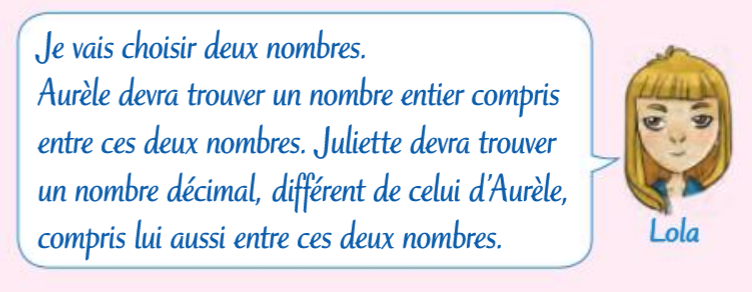
\includegraphics[scale=0.7]{img/lola}
\end{center}

\begin{questions}
	\question[1] Lola a choisi  \num{322.1} et \num{325.4}. Donner toutes les réponses possibles pour Aurèle et dix réponses possibles pour Juliette.
	
	\question[1] Lola choisi tà présent \num{12.3} et \num{12.4}. Donner toutes les réponses possibles pour Aurèle et dix réponses possibles pour Juliette.Peut-on donner toutes les réponses possibles ?
	
	
\question[1] Aurèle n'est pas content et dit à Lola que ses règles du jeu sont injustes. Expliquer pourquoi.
\end{questions}

\section{Somme de deux nombres (Bonus)}

Jules et Samia n'arrivent pas à se mettre d'accord sur l'énoncé suivant :

<< La somme de deux nombres est toujours plus grande que chacun de ces nombres.>>

Samia dit que c'est faux alors que Jules insiste pour dire que c'est vrai.

\begin{questions}
	\question Aider ces deux élèves à se mettre d'accord.
\end{questions}



\label{LastPage}

%\section{Consommation électrique}
%
%Une consommation d'électricité se mesure en 
\end{document}